\documentclass[20pt,a4paper,landscape]{extarticle}
\usepackage[margin=1.25in]{geometry}
\usepackage{placeins}
\usepackage{latexsym}
\usepackage{marvosym}
\usepackage[utf8]{inputenc}
\usepackage[T1]{fontenc}
\usepackage[UKenglish]{babel}
\usepackage[UKenglish]{isodate}
\usepackage{amsmath}
\usepackage{amsfonts}
\usepackage{amssymb}
\usepackage{amsthm}
\usepackage{graphicx}
\usepackage{titletoc}
\usepackage{listings}
\usepackage{dsfont}
\usepackage{changepage}
\usepackage{lpform}
\usepackage{tikz}
\usetikzlibrary{arrows.meta, mindmap, trees, shapes.geometric, positioning, matrix}
\lstset{
    basicstyle=\ttfamily,
    mathescape
}
\PassOptionsToPackage{hyphens}{url}
\usepackage{xurl}
\input{glyphtounicode}
\pdfgentounicode=1
\usepackage[all]{nowidow}
\usepackage{hyperref}
\hypersetup{
        colorlinks,
        citecolor=black,
        filecolor=black,
        linkcolor=black,
        urlcolor=black
}
\usepackage[protrusion=true,expansion=true]{microtype}
\newcommand{\ind}{\perp\!\!\!\!\perp}
\newcommand{\Obj}{\textrm{Obj}}
\renewcommand{\th}[1]{#1^\textrm{th}}
\let\max\relax
\DeclareMathOperator*{\max}{max\:}
\let\min\relax
\DeclareMathOperator*{\min}{min\:}
\DeclareMathOperator*{\argmax}{arg\,max\:}
\DeclareMathOperator*{\argmin}{arg\,min\:}
\begin{document}
\tableofcontents
\clearpage
\begin{flushleft}
\section{Introduction to Approximation Algorithms}
\subsection{Approximation}
\begin{itemize}
\item An algorithm for an optimization problem must always return a feasible solution but no guarantee is provided about the objective function value for the returned solution
\item \textbf{Approximation ratio $\alpha$ of an algorithm $A$ = for the worst input $I$, $\frac{\Obj(A(I))}{\Obj(OPT(I))}$}
\item For a maximization problem, $0 \leq \alpha \leq 1$. For a minimization problem, $\alpha \geq 1$. For an optimal algorithm, $\alpha = 1$ (for both objective types)
\end{itemize}
\subsection{Greedy approximation}
\subsubsection{Set Covering}
\begin{itemize}
\item \textbf{MAXIMUM-COVERAGE = Given a universe $U$ of $n$ elements and $m$ sets $S_1, ..., S_m \subseteq U$, pick $k$ sets from $\{S_1, ..., S_m\}$. Call an element of $U$ covered iff it is in the union of the chosen k sets. Choose so as to maximize the number of covered elements}
\item Computing all $m\textrm{C}k$ sets to check will take $O(m^k)$ time, so is not polynomial time as k is a parameter of the input
\item We present a greedy algorithm for a generalisation of this problem where each covered element has an integer payoff $p_i \in [1, n]$:\\
\begin{lstlisting}
R = $\emptyset$
T = $\{\mathtt{S}_1, ..., \mathtt{S}_\mathtt{m}\}$
C = $\emptyset$
for $t \in [k]$
    Pick $S_\mathtt{i} \in \underset{S_\mathtt{i} \in \mathtt{T}}{\argmax}(\underset{e_j \in S_\mathtt{i} - \mathtt{C}}{\sum} w_j)$
    R $\cup$= $\{S_\mathtt{i}\}$
    T $\setminus$= $\{S_\mathtt{i}\}$
    C $\cup$= $S_\mathtt{i}$
return R
\end{lstlisting}
Theorem: \textbf{Let $\alpha$ be the approximation ratio of this algorithm. Then, $\alpha \geq 1 - \frac{1}{e}$}\\
Proof: Exercise (problem from assessed assignment)\\
\textbf{Lemma: If $t \in \mathbb{N}_{>0}$ and $k \geq t$, then $(1 - \frac{1}{k})^t \leq e^{-\frac{t}{k}}$}\\
\textit{Proof:
The Maclaurin series for $e^x$ has infinite radius of convergence. As $t$ is a positive integer, the binomial series for $(1+x)^{t}$ is convergent for all $x$.\\
$e^{-\frac{t}{k}} = \sum_{n=0}^{\infty}\left(\left(\frac{-t}{k}\right)^n\left(\frac{1}{n!}\right)\right)$\\
$\left(1 - \frac{1}{k}\right)^t = \sum_{n=0}^{t}\left(\left(\frac{-1}{k}\right)^n\left(\frac{t!}{(t-n)!n!}\right)\right) \leq \sum_{n=0}^{t}\left(\left(\frac{-1}{k}\right)^n\left(\frac{t^n}{n!}\right)\right) = \sum_{n=0}^{t}\left(\left(\frac{-t}{k}\right)^n\left(\frac{1}{n!}\right)\right)$.\\
As $t \leq k$, $\left(\frac{t}{k}\right)^n$ is a decreasing function of n. Hence, $\left(1 - \frac{1}{k}\right)^t \leq \sum_{n=0}^{t}\left(\left(\frac{-t}{k}\right)^n\left(\frac{1}{n!}\right)\right) \leq \sum_{n=0}^{\infty}\left(\left(\frac{-t}{k}\right)^n\left(\frac{1}{n!}\right)\right) = e^{-\frac{t}{k}}$}
\end{itemize}
\subsubsection{Centroids}
\begin{itemize}
\item \textbf{K-Centre = Given $V=\{1, ..., n\}$, a metric $d: V^2 \mapsto \mathbb{R}_{>0}$, and $k \leq n$, find a $S \subseteq V$ subject to $|S|=k$ that minimizes $\underset{j \in V}{\max}d(j, S)$}
\item A greedy algorithm: Pick an arbitrary initial point to add to S. For the remaining $k-1$ members of $S$, at each step chose the point that is furthest away from its nearest point in the current $S$
\item Theorem: \textbf{The above algorithm is a 2-approximation}\\
Proof: $S$ can be seen to partition $V$ with each point in $V$ being a member of the cluster represented by the nearest point in $S$ to it. Let the radius of a cluster be the point in that that is the furthest away from its centre (the member of $S$ that belongs to it (and it was constructed from)).\\
Base case $k=1$: The point is chosen completely arbitrarily, this may seem suspect but we will show it is fine. Let $j^\ast, r^\ast$ be the centre and radius of an optimal solution. Then, every point in $V$ is at most $r^\ast$ away from $j$. Let $j$ be the centre picked by greedy. Pick an arbitrary point $i \in V$, as $d$ is a metric it obeys the triangle inequality, thus $d_{ij} \leq d_{ij^\ast} + d_{j^\ast j} \leq r^\ast + r^\ast = 2r^\ast$ as required.\\
Inductive step $k=m+1$: Let $S^\ast = \{j_1, ..., j_k\}$ be the centres chosen by an optimal solution and $r^\ast$ be the largest radius in $S$. If every cluster chosen by greedy is in a distinct cluster in $S$, then the necessary bound easily follows from the obvious generalisation of the argument in the $k=1$ case. Otherwise, still by the same fundamental argument, the distance between two points (such as those chosen by greedy) in the same cluster must be at most $2r^\ast$, and the fact that greedy went on to pick the second of the points it picked witnesses that there cannot be any points in $V$ further away from this cluster than this (otherwise they would've been greedily chosen in its place), thus we have the required result.
\end{itemize}
\clearpage
\section{Linear Programming}
\subsection{LP Relaxation}
\begin{itemize}
\item Most optimization problems can be represented as an integer program (IP). Integer programming is NP-Hard, but by relaxing the integrality constraints we get a linear program (LP). With a rounding scheme, we can obtain, from an LP, approximately optimal solutions to an IP in polynomial time
\item $\min\underset{a \in A}{\max}f(a) = \min T$ subject to ($f(a) - T \leq 0 \; \forall a \in A$)
\item Deduce that the set of feasible solutions to an LP relaxation is a superset of the set of feasible solutions to the IP. Thus, deduce that the value of optimal solutions to the LP (allowing fractional solutions) is at least as good as the value of optimal solutions to the IP
\item \textbf{Integrality gap = for the worst input $I$, $\frac{IP_{OPT}(I)}{LP_{OPT}(I)}$}. This lower bounds the approximation ratio of any rounding scheme
\item Relationships in a maximization problem:
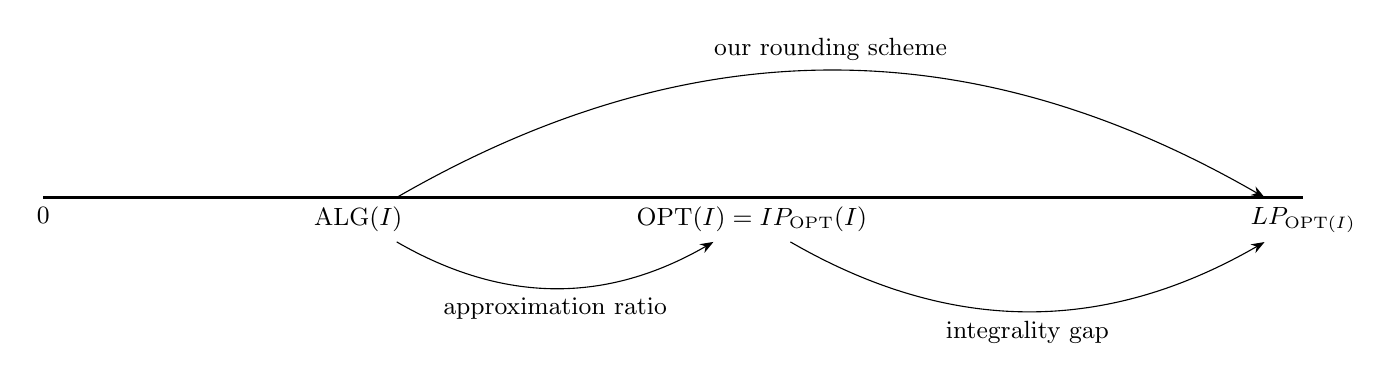
\begin{tikzpicture}[>=Stealth, node distance=3cm, every node/.style={font=\small}]
\draw[thick] (0,0) -- (16,0);
\node[below] (zero) at (0,0) {0};
\node[below] (alg) at (4,0) {$\mathrm{ALG}(I)$};
\node[below] (opt) at (9,0) {$\mathrm{OPT}(I) = IP_{\mathrm{OPT}}(I)$};
\node[below] (lp) at (16,0) {$LP_{\mathrm{OPT}(I)}$};
\draw[->, bend left=30] (alg) to node[above, midway, align=center] {our rounding scheme} (lp);
\draw[->, bend right=30] (alg) to node[below, midway, align=center] {approximation ratio} (opt);
\draw[->, bend right=30] (opt) to node[below, midway, align=center] {integrality gap} (lp);
\end{tikzpicture}
\end{itemize}
\clearpage
\subsection{LP Rounding}
\item Proposition: The best approximation for minimum vertex-cover obtainable by LP rounding is exactly a 2-approximation\\
Proof: The following is the LP relaxation:
\begin{lpformulation}
\lpobj*{min}{|S(z)| = \sum_{v \in V} x_v}
\lpeq*{x_u + x_v \geq 1}{(u, v) \in E}
\lpeq*{0 \leq x_v \leq 1}{v \in V}
\end{lpformulation}
Lemma: Integrality gap $\geq 2$. Thus, $\alpha \geq 2$\\
Proof: Consider the complete graph $K_n$. $LP_{OPT} = \frac{n}{2}$ (chose every node but only ``half'' chose them) whereas $IP_{OPT} = n-1$ (chose every node except for one). As this is a particular case, it acts as a lower bound on the integrality gap. Finally, $\frac{2(n-1)}{n} \to 2$ when $n \to \infty$\\
\clearpage
Lemma: $\alpha \leq 2$. Thus, $\alpha = 2$\\
Proof: Use ordinary rounding: $\geq 0.5 \mapsto 1$, $< 0.5 \mapsto 0$. This is a legal rounding scheme as every feasible solution to the LP will when rounded be a feasible solution to the IP as $x_u + x_v \geq 1 \land x_u, x_v \leq 1 \Rightarrow$ $x_u \geq 0.5 \lor x_v \geq 0.5$. Each term in the objective at most doubles under this rounding scheme, thus $IP_{OPT} \geq 2 LP_{OPT}$ (as our rounding scheme gives a feasible solution to $IP$). Finally, as $IP_{OPT} = OPT$, $OPT \geq 2 LP_{OPT}$ as required)
\subsection{Duality}
\begin{itemize}
\item An LP can be converted to standard form by:
    \begin{itemize}
    \item Constraints $\leq$ for $\min$ (so $\geq$ for $\max$): $Cx = b \Rightarrow$\\
    $cx \leq b$ and $cx \geq b$ $\Rightarrow$ $cx \leq b$ and $-cx \leq -b$
    \item Make variables non-negative: $x \rightarrow x^+ - x^-$ and $x^+, x^- \geq 0$
    \end{itemize}
\begin{lpformulation}
\lpobj*{min}{c_1x_1 + ... + c_nx_n}
\lpeq*{a_{11}x_1 + ... + a_{1n}x_n \geq b_1}{}
\lpeq*{...}{}
\lpeq*{a_{m1}x_1 + ... + a_{mn}x_n \geq b_m}{}
\lpeq*{x_1, ..., x_n \geq 0}{}
\end{lpformulation}
$\underset{\textrm{dual}}{\Leftrightarrow}$
\begin{lpformulation}
\lpobj*{max}{b_1y_1 + ... + b_my_m}
\lpeq*{a_{11}y_1 + ... + a_{m1}y_m \leq c_1}{}
\lpeq*{...}{}
\lpeq*{a_{1n}y_1 + ... + a_{mn}y_m \leq c_n}{}
\lpeq*{y_1, ..., y_m \geq 0}{}
\end{lpformulation}
\item Weak duality theorem: Let $LP_1$ be the primal and $LP_2$ be the dual. Assume without loss of generality that $LP_1$ is a minimization problem. Then, $OPT_2 \leq OPT_1$\\
Proof: Out of scope (see MA252 if interested)
\item \textbf{Strong duality theorem: optimal value of primal = optimal value of dual}\\
Proof: Out of scope
\item \textbf{Complementary slackness theorem: A pair of feasible solutions to primal and dual are both optimal $\Leftrightarrow$ whenever a primal-variable is non-zero the corresponding dual-constraint is tight and whenever a dual-variable is non-zero the corresponding primal-constraint is tight}\\
Proof: Out of scope (see MA252 if interested)
\clearpage
\item \textbf{Approximate complementary slackness theorem: Call a constraint $ax \geq b$ $\alpha_1$-tight ($\alpha_1 \geq 1$) iff $\alpha_1 b \geq ax \geq b$ and a constraint $ax \leq b$ $\alpha_2$-tight ($\alpha_2 \geq 1$) iff $\frac{b}{\alpha_2} \leq ax \leq b$. Let $x^\ast, y^\ast$ be feasible solutions to primal and dual respectively.\\
If (there exists $\alpha, \beta \geq 1$ such that whenever a variable in $x^\ast$ is non-zero, the corresponding dual constraint is $\alpha$-tight and whenever a variable in $y^\ast$ is non-zero, the corresponding primal constraint is $\beta$-tight), then the multiplicative factor between \Obj$(x^\ast)$ and \Obj$(y^\ast)$ is at most $\alpha\beta$}\\
Proof: Out of scope
\end{itemize}
\clearpage
\subsection{Dual Fitting}
\begin{itemize}
\item Whereas LP rounding is an approach for \underline{constructing} an approximation algorithm, dual fitting is an approaching for \underline{analysing} the approximation ratio of a given approximation algorithm (for example, a greedy algorithm for a certain problem)
\item \textbf{As any approximation algorithm gives feasible solutions to the problem, it gives feasible solutions to an LP relaxation of the problem. If we can demonstrate an upper bound on the objective function value gap between this feasible solution to the primal LP and a feasible solution to the dual LP}, this will also be an upper bound on the approximation ratio as for every pair of feasible primal and dual solutions the (shared) optimal value lies between them (and the optimal value for the IP and so the true problem is no better than that of the LP relaxation).
\clearpage
\item Theorem: At each step picking the set that contains the most uncovered elements is a $\log n$-approximation for set-cover\\
Proof: Let $\hat{S}_j$ = the set of elements newly covered in iteration $j$\\
The LP relaxation for MIN-SET-COVER is:
\begin{lpformulation}
\lpobj*{min}{|I| = \sum_{k \in [m]} x_j}
\lpeq*{\sum_{j: e_i \in S_j} x_j \geq 1}{i \in [n]}
\lpeq*{0 \leq x_j \leq 1}{j \in [m]}
\end{lpformulation}
\clearpage
In standard form (with extraneous $x_j \leq 1$ constraint dropped):
\begin{lpformulation}
\lpobj*{min}{\sum_{k \in [m]} x_j}
\lpeq*{\sum_{j: e_i \in S_j} x_j \geq 1}{i \in [n]}
\lpeq*{x_j \geq 0}{j \in [m]}
\end{lpformulation}
Thus, the dual is:
\begin{lpformulation}
\lpobj*{max}{\sum_{i \in [n]} y_i}
\lpeq*{\sum_{i: e_i \in S_j} y_i \leq 1}{j \in [m]}
\lpeq*{y_i \geq 0}{i \in [n]}
\end{lpformulation}
\textit{The dual corresponds to the fractional packing problem: Assign a positive value to each element in the universe to maximize the total value of the universe under the constraint that the total value of each set is at most one.}\\
There must exist a feasible LP solution $P$ with objective value the same as the greedy algorithm solution. We will show that $P$ induces a feasible dual solution $D$ such that $P \leq O(\log n)D$. Then, as $D \leq OPT$, $P \leq O(\log n)OPT$ as required.\\
In particular, $x_k = 1$ iff $S_j$ is chosen by greedy; 0 otherwise is a suitable $P$. A natural corresponding dual solution is then $y_i = \frac{1}{|\hat{S}_l|} \forall e_i \in S_l; \forall l \in [k];$ [as each element is only newly covered in one iteration this is well defined]. However, we constructed this to have exactly the same objective value as $P$, thus it must be not in general feasible (as dual and primal only coincide for optimal solutions (and solving this problem optimally is NP-Hard)), so we need to tweak it.\\
The constraints are that $\sum_{i: e_i \in S_j} y_i \leq 1$, whereas we will be able to show that $\sum_{i: e_i \in S_j} y_i \leq O(\log n)$. Thus, dividing every variable in $D$ by $O(\log n)$ will give a feasible dual solution with value only a multiplier of $O(\log n)$ away from $P$ as required.\\
Pick an arbitrary $S_j$ from the set of allowed sets. Let $X_t$ = the set of elements that are newly added in the $\th{t}$ iteration of greedy and are in $S_j$. Let $n_t = |X_t|$. Then, $|S_j| = \sum_{t \in [k]} n_t$ where $k$ is the value of the greedy solution. Pick an arbitrary iteration $t$ of greedy. Then, $X_t = \hat{S}_t \cap S_j$. By the greediness, $|\hat{S}_t| \geq |S_j \setminus \left(X_1 \cup ... X_{t-1}\right)|$, as $S_t$ was chosen instead of $S_j$. Note that, $|S_j \setminus \left(X_1 \cup ... X_{t-1}\right)| =$\\
$ n_1 + ... + n_k - n_1 - ... - n_{t-1} = n_t + ... + n_k$. Thus, $|\hat{S}_t| \geq \sum_{l=t}^k n_l$. Therefore, $\sum_{e_i \in X_t} y_i \leq \frac{n_t}{n_t + ... + n_k}$. Thus, $\sum_{e_i \in S_j} \leq \sum_{t=1}^k \frac{n_t}{\sum_{z=t}^k n_z} \leq \sum_{z=0}^{N-1} \frac{1}{N-z} \in O(\log N)$ where $N = |S_j|$. As $S_j \subseteq U$ and $n = |U|$, we have our desired $O(\log n)$ bound.
\end{itemize}
\clearpage
\section{Randomized algorithms}
\subsection{Derandomisation}
Some randomized algorithms can be rewritten as a deterministic algorithm of the form:
\begin{lstlisting}
for $i \in \{1, n\}$
    Pick a value for $\alpha_i$ such that
    $E[f(X_1, ..., X_n)|X_1=\alpha_1, ..., X_i=\alpha_i]\geq B$
return solution induced by $X_1=\alpha_1, ..., X_n=\alpha_n$
\end{lstlisting}
where $E[f(X_1, ..., X_n)|\emptyset]\geq B$.

For these, the \underline{deterministic} value of our solution is at least $B$ as we have this for the empty solution at the start of the loop and each iteration of the loop preserves the invariant that the partial solution obeys this. By an averaging argument, there exists a suitable $\alpha_i$ at every step by induction.\\
Human analysis of the structure of the problem is required to demonstrate a deterministic polynomial time algorithm for choosing such an $\alpha_i$ at each step
\subsection{Karger's Algorithm}
\begin{itemize}
\item Karger's algorithm finds a minimum cut in near-linear time ($\widetilde{O}(n)$ ($O(m\cdot\text{poly}(\log n)$))). \textit{This problem can be solved deterministically in polynomial time using maximum flow algorithms but by randomization Karger was able to obtain near-linear time}
\item An edge contraction merges two nodes into one, making the obvious changes to the edges. Where both nodes had edges incident on them from the same node, there will be two edges from this to the new node. \textbf{The algorithm is simply to pick \underline{uniformly} at random which edge to contract until there are only two nodes remaining then return the induced cut} (the two ``supernode''s at the end partition the graph and so are a cut). Edges which have multiple copies thus have a higher chance of being chosen
\item With suitable data structures, edge contraction can be done in $\widetilde{O}(n)$ time. There are exactly $n-1$ contractions to do. Thus, the entire algorithm takes $\widetilde{O}(n^2)$  time, which is near-linear time as the size of the edges of a general graph is $O(n^2)$
\item Theorem: \textbf{Karger gives an optimal solution with probability at least $\frac{1}{n\textrm{C}2 \in \Theta(n^2)}$}\\
Proof: \textbf{Pick an arbitrary minimum cut $S^\ast$. We will actually be able to show that this exact cut is chosen with this probability bound.}\\
Let $k = |\delta(S^\ast)| =$ the size of a min-cut and $G_i = (V_i, F_i) =$ the super-graph at the \underline{beginning} of iteration $i$. Say that a cut S survives iteration $i$ iff $\delta(S) \subseteq E_{i\underline{+1}}$ (none of the cut's edges have been absorbed inside a super node (they are all between super-nodes at the start of iteration $i+1$)). Deduce that $S$ survives iteration $j$ iff $S$ survives iterations $1, ..., j-1$ and the super-edge contracted in iteration $j$ is in $E_i \setminus \delta(S)$.\\
Deduce that $S^\ast$ is chosen iff $S^\ast$ survives iteration $n-2$. Let $H_i = 1$ iff $S^\ast$ survives iteration $i$. Then, by the law of total probability, $\Pr(H_{n-2}) =$\\
$\prod_{i=1}^{n-2} \Pr(H_i | H_1 \cap ... \cap H_{i-1})$.\\
Lemma: minimum degree in $G_i \geq$ size of min-cut in $G_i \geq$ size of min-cut in $G = k$\\
Proof:
\begin{adjustwidth}{1em}{}
size of min-cut in $G_i \geq$ size of min-cut in $G$ is trivial and $k=$ size of min-cut in $G$ is the definition of $k$. It remains to show that minimum degree in $G_i$ $\geq$ size of min-cut in $G_i$. In any graph, a minimum cut is a witness to a lower bound on the minimum degree (as a node with smaller degree would alone be a cut with fewer edges), so we have the required result.
\end{adjustwidth}
In iteration $i$ we chose an edge from $E_i$ to contract. By the infamous handshaking-lemma $\left(|E_i| = \frac{1}{2}\sum_{v \in V(G_i)} \textrm{degree}(v)\right)$, deduce that $|E_i| \geq \frac{|V_i|}{2}\textrm{min\_degree}(G_i)$ . Moreover, we have already argued that $\textrm{min\_degree}(G_i) \geq k$. Finally, as the algorithm does exactly one edge contraction per iteration, $|V_i| = n-i+1$. Thus, $|E_i| \geq \frac{k}{2}(n-i+1)$.\
Thus, $\Pr(H_i = 0 | H_1 = ... H_{i-1} = 1) \leq \frac{k}{\frac{k}{2}(n-i+1)} = \frac{2}{n-i+1}$. Thus, $\Pr(H_i = 1 | H_1 = ... H_{i-1} = 1) \geq 1 - \frac{2}{n-i+1} = \frac{n-i-1}{n-i+1}$.\\
Thus, $\Pr(H_{n-2}) \geq \frac{n-2}{n}\frac{n-3}{n-1}\frac{n-4}{n-2}...\frac{1}{3} = \frac{2}{n(n-1)}$ [telescoping] $= \frac{1}{n\textrm{C}2}$ as required
Corollary (cut-counting lemma): No graph has more than $n^2$ distinct min-cuts
\clearpage
\item We can apply probability amplification: If the algorithm is ran $c \cdot \log n \cdot n \textrm{C}2$ times and the smallest cut from all the trials is returned, then we take $\widetilde{O}(n^2)$ (remember this is actually only quadratic in the input size of general graphs) time and have success probability of at least $1-(1-\frac{1}{n\textrm{C}2})^{c\cdot\log (n)\cdot n\textrm{C}2} \approx 1 - \left(\frac{1}{e}\right)^{c \cdot \log n}$ [Taylor series for $(1-\frac{1}{a})^a$]\\
$= 1 - \frac{1}{n^c}$. \textbf{We call anything that goes to 1 at least as fast as $1 - \frac{1}{n}$ ``with very high probability''}
\end{itemize}
\clearpage
\section{Probability}
\subsection{Bounds}
\item \textbf{Union bound: $\forall E_1, ..., E_n; \Pr(E_1 \cup ... \cup E_n) \leq \Pr(E_1) + ... + \Pr(E_n)$}\\
Proof: CS275
\item \textbf{Linearity of expectation: $\forall X_1, ..., X_n; E[X_1 + ... + X_n] = E[X_1] + ... + E[X_n]$}\\
Proof: CS275
\item \textbf{Markov's Inequality: Let $X$ be a \underline{non-negative} discrete random variable and $a$ be a \underline{positive} number. Then, $\Pr(X \geq a) \leq \frac{E[X]}{a}$}. Or equivalently (and more intuitively), $\Pr(X \geq E[X]a) \leq \frac{1}{a}$\\
Intuition: Averaging argument (CS301)\\
Proof: Let $Y$ = 1 iff $X \geq a$, 0 otherwise. Then, $Y \leq \frac{X}{a}$. Thus, $E[Y] \leq E[\frac{X}{a}] = \frac{E[X]}{a}$. Finally, $E[Y] = \Pr(Y = 1) = \Pr(X \geq a)$
\clearpage
\item \textbf{Chernoff bound: If $X = \sum_{i=1}^n X_i$ and $X_i$ are all \underline{mutually independent} \underline{and $\{0, 1\}$-valued} and $0 < \delta < 1$, then $\Pr(X \geq (1 + \delta)E[X]) \leq \exp(\frac{-E[X]\delta^2}{3})$ [this direction also works for $\delta = 1$] and $\Pr(X \leq (1 - \delta)E[X]) \leq \exp(\frac{-E[X]\delta^2}{2})$}\\
Proof for $\geq$: Consider $Y=\exp(\ln(1+\delta)X)$. Then, $\Pr(X \geq (1+\delta)E[X]) =$\\
$\Pr(Y \geq \exp(\ln(1+\delta)(1+\delta)E[X])$.\\
Lemma: $\forall i \in [n];\; E[\exp(\ln(1+\delta)X_i)] \leq \exp(\Pr(X_i=1)(\exp(\ln(1+\delta))-1))$\\
Proof:
\begin{adjustwidth}{1em}{}
$E[\exp(\ln(1+\delta)X_i)] = \Pr(X_i=1)\exp(\ln(1+\delta)) + \Pr(X_i=0) \cdot 1 =$\\
$\Pr(X_i=1)\exp(\ln(1+\delta)) + 1 - \Pr(X_i=1) =$\\
$\Pr(X_i=1)(\exp(\ln(1+\delta)) - 1) + 1 \leq \exp(\Pr(X_i=1)(\exp(\ln(1+\delta))-1))$ [as $e^k \geq k+1\;\forall k \in \mathbb{R}$]
\end{adjustwidth}
Lemma: $E[Y] \leq \exp(\delta E[X])$\\
Proof:
\begin{adjustwidth}{1em}{}
By grade-school algebra, $Y = \exp(\ln(1+\delta)X_1+...+\ln(1+\delta)X_n) =$\\
$\exp(\ln(1+\delta)X_1)...\exp(\ln(1+\delta)X_n)$. Thus, as the $X_i$s are independent, $E[Y] = E[\exp(\ln(1+\delta)X_1)]...E[\exp(\ln(1+\delta)X_n)]$. So, by the previous lemma, $E[Y] \leq \exp((\Pr(X_1=1)+...+\Pr(X_n=1))(\exp(\ln(1+\delta))-1))$.\\
As $X$ is the sum of $\{0, 1\}$-valued random variables, $E[X] = \Pr(X_1=1)+...+$\\
$\Pr(X_n=1)$. Thus, $E[Y] \leq \exp((\exp(\ln(1+\delta))-1)E[X]) =$\\
$\exp((1+\delta-1)E[X]) = \exp(\delta E[X])$\\
\end{adjustwidth}
By Markov's inequality, $\Pr(Y \geq \exp(\ln(1+\delta)(1+\delta)E[X])) \leq$\\
$\frac{E[Y]}{\exp(\ln(1+\delta)(1+\delta)E[X])} = \frac{E[Y]}{(1+\delta)^{(1+\delta)^{E[X])}}}$. Thus, by our bound on $E[Y]$, $\Pr(X \geq (1+\delta)E[X]) \leq \frac{e^{\delta^{E[X]}}}{(1+\delta)^{(1+\delta)^{E[X])}}} = \left(\frac{e^\delta}{(1+\delta)^{(1+\delta)}}\right)^{E[X]}$\\
Lemma: $\forall 0 < \delta \leq 1; \; \frac{e^\delta}{(1+\delta)^{(1+\delta)}} \leq e^{-\frac{\delta^2}{3}}$\\
Proof: Out of scope\\
By the above lemma (and elementary indices laws), $\Pr(X \geq (1+\delta)E[X]) \leq e^{-E[X]\left(\frac{\delta^2}{3}\right)}$ as required.\\
Proof for $\leq$: Exercise
\subsection{Randomized LP Rounding}
\subsubsection{Randomized rounding framework}
\textbf{
\begin{enumerate}
\item Show that there are at most polynomial many bad events and none of the bad events occurring is sufficient for a solution to be valid. Define good events the complements of the bad events: then there are most polynomially many of these and all the good events occurring is sufficient for a solution to be valid
\item Show that each good event occurs with high probability (for example using a Chernoff bound) i.e. that each bad event occurs with probability at most $\frac{1}{\textrm{poly}(n)}$
\item Thus, by the union bound, all the good events occurring together is also with high probability. Thus, the algorithm gives a feasible solution with high probability
\item Take expectation of value and thus deduce expectation of approximation ratio. If possible, strengthen to actual value of approximation ratio obeying this with high probability
\end{enumerate}
}
\subsubsection{FACILITY-LOCATION}
FACILITY-LOCATION = Given $F=\{1, ..., m\}$, $C=\{1, n\}$, $f \in \mathbb{R}^m_{\geq 0}$, $d \in \left(\mathbb{R}_{\geq 0}\right)_{m \times n}$, find $H \subseteq F$ and $a \in H^n$ that minimizes $\sum_{i \in H}f_i + \sum_{j \in C}d_{a_j, i}$. This is a generalisation of minimum-set-cover, so every approximation algorithm for this is an upper bound on the approximation ratio of minimum-set-cover.\\
LP relaxation:
\begin{lpformulation}
\lpobj*{min}{\sum_{i \in F} x_if_i + \sum_{i \in F} \sum_{j \in C} y_{ij}d_{ij}}
\lpeq*{y_{ij} \leq x_i}{i \in F. \forall j \in C}
\lpeq*{x_i \leq 1}{i \in F}
\lpeq*{y_{ij} \leq 1}{i \in F. \forall j \in C}
\lpeq*{x_{i} \geq 0}{i \in F}
\lpeq*{y_{ij} \geq 0}{i \in F. \forall j \in C}
\end{lpformulation}
Randomized rounding scheme:
\begin{lstlisting}
for $i \in F$
    Sample $\tau_i$ from 0--1 uniformly at random
    Open $i$ iff $\left(K \log n\right) x_i^\ast \geq \tau_i$
    for $j \in C$
        Connect $j$ to $i$ iff $\left(K \log n\right) y_{ij}^\ast \geq \tau_i$
\end{lstlisting}
Let $p_i$ = probability facility $i$ is opened, then $p_i = \min(1, \left(K \log n\right) x_i^\ast)$. Similarly, $q_{ij}$ = probability client $j$ is connected to facility $i$ = $\min(1, \left(K \log n\right) y_{ij}^\ast)$.\\
As $y_{ij}^\ast \leq x_i^\ast$ by the LP constraint, $\left(K \log n\right) y_{ij}^\ast \leq \left(K \log n\right) x_i^\ast$. Thus, if $j$ is assigned to $i$, then $\tau_i \leq \left(K \log n\right) y_{ij}^\ast$ and so by transitivity $\tau_i \leq \left(K \log n\right) x_i^\ast$. That is that every assignment of a client to a facility is to an open facility.\\
We will show shortly that every client is assigned to at least one open facility with high probability (and thus the rounded solution is feasible with high probability).\\
Before that, we will show that, in expectation, this rounding is an $\Theta(\log n)$- approximation. $E[$objective function of greedy$] = E[\sum_{i \in F} f_ix_i + \sum_{i \in F} \sum_{j \in C} d_{ij}y_{ij}] = \sum_{i \in F} f_iE[x_i] + \sum_{i \in F} \sum_{j \in C} d_{ij}E[y_{ij}] = \sum_{i \in F} f_i \Pr(x_i = 1) + \sum_{i \in F} \sum_{j \in C} d_{ij} \Pr(y_{ij = 1}) \leq \sum_{i \in F} f_i\left(K \log n\right) x_i^\ast + \sum_{i \in F} \sum_{j \in C} d_{ij}\left(K \log n\right) y_{ij}^\ast) = \left(K \log n\right)LP_{OPT} = \Theta(\log n)LP_{OPT}$. Finally, as $LP_{OPT} \leq OPT$ and greedy $\leq \Theta(\log n)LP_{OPT}$, greedy $\leq \Theta(\log n)OPT$ as required.\\
Now we will finish the proof of the feasibility. Pick arbitrary $j \in C$. $\Pr(j$ is not assigned to any facility$)$ = $\Pr(\bigcap_{i \in  F}j$ is not assigned to facility $i) = \prod_{i \in  F} \Pr(j$ is not assigned to facility $i)$ [as these events are independent as they depend only on the $\tau_i$s which are themselves independent] $= \prod_{i \in  F}\left(1 - \min\left(1, \left(K \log n\right) y_{ij}^\ast\right)\right) \leq \prod_{i \in  F}\left(1 - \left(K \log n\right) y_{ij}^\ast\right) \leq \prod_{i \in  F}\exp\left(- \left(K \log n\right) y_{ij}^\ast\right)$ \textbf{[as $1-x \leq e^{-x}$]} $= \exp\left(- \left(K \log n\right) \sum_{i \in F} y_{ij}^\ast\right)$ [$x^yx^z = x^{y+z}$] $\leq \exp\left(- \left(K \log n\right)\right)$ [LP constraint] $= \frac{1}{n^K}$. We have shown that $\Pr(j$ is not assigned to any facility$) \leq \frac{1}{n^K}$ for every client $j$\\
By the union bound, $\Pr($some client is not assigned to any facility$) \leq \frac{n}{n^K} = \frac{1}{n^{K-1}}$. Finally, by complementation, $\Pr($every client is assigned at least one facility$) \geq 1 - \frac{1}{n^{K-1}}$ which is with high probability for $K \geq 2$ and $K$ was free for us to choose.
\subsection{Coupon Collector}
\textbf{Coupon collector theorem: In each step, a coupon is drawn uniformly at random from a bucket of $n$ coupons then returned to the bucket. The expected number of steps until every coupon has been seen (at least) once is $\Theta(n \log n)$}\\
Proof: Let $X_i$ = number of steps between $\th{(i-1)}$ new coupon seen and $\th{i}$ coupon seen. Let $X=$ number of steps until every coupon has been seen. Then, $X = \sum_i X_i$. By linearity of expectation, $E[X] = \sum_{i \in [n]} E[X_i]$. After seeing the $\th{(i-1)}$ new coupon, there are $n-(i-1) = n-i+1$ coupons not yet seen. Thus, at every step while waiting, the probability of stopping is $\frac{n-i+1}{n}$. That is that $X_i \sim \textrm{Geometric}(\frac{n-i+1}{n})$. Thus, $E[X_i] = \frac{1}{\frac{n-i+1}{n}} = \frac{n}{n-i+1}$.\\
Thus, $E[X] = \sum_{i \in [n]} \frac{n}{n-i+1} = \sum_{j \in [n]} \frac{n}{j}$ [by reordering terms for cleaner indexing]. \textbf{By harmonic series, $\sum_{j \in [n]} \frac{1}{j}\in \Theta(\log n)$}. Thus, $E[X] \in \Theta(n \log n)$ as required.
\subsection{Balls into Bins}
\begin{itemize}
\item We have $m$ balls each of which falls uniformly at random into one of $n$ bins
\item \textbf{We say that balls $i$ and $j$ ($i \neq j$) collide iff $i$ and $j$ land in the same bin} (note that balls are not considered to be ordered within a bin).\\
$\Pr($balls $i$ and $j$ collide$)$ = $\bigcup_{k \in [n]} \Pr($balls $i$ and $j$ are both in bin $k)$ = $\sum_{k \in [n]}$ $\Pr($balls $i$ and $j$ are both in bin $k)$ [as are mutually exclusive] = $n\frac{1}{n}\frac{1}{n}= \frac{1}{n}$
\item Expected number of collisions =\\
E$[\sum_{i \in [n]} \sum_{j \in [n]: j \neq i} 1\times\Pr($balls $i$ and $j$ collide$)$] =\\
$\sum_{i \in [n]} \sum_{j \in [n]: j \neq i} \frac{1}{n}$ [by linearity of expectation] = $\left(m\textrm{C}2\right)\frac{1}{n}$
\clearpage
\item \textit{Birthday paradox: Suppose m people's birthdays are uniformly distributed across 365 days of the year (sorry leaplings). Then, expected number of shared birthdays = $\frac{m^2 - m}{2\times365} \geq 1$ if $m \geq 27$. Similarly, $\Pr($there is at least one shared birthday$)$ = $\left(1-\frac{1}{365}\right)^{m\textrm{C}2} \geq \frac{1}{2}$ iff $\frac{m^2-m}{2} \geq \frac{\ln\left(\frac{1}{2}\right)}{\ln\left(1 - \frac{1}{365}\right)}$ if $m \geq 23$}
\item $\Pr($bin $k$ is empty$)$ = $\bigcap_{i \in [m]} \Pr($ball $i$ did not fall into bin $k)$ = $(1-\frac{1}{n})^m$ [as balls are independent from each other] $\leq e^\frac{-n}{m}$ and $\rightarrow e^\frac{-n}{m}$ as $n \rightarrow \infty$ or $m \rightarrow \infty$. Thus, by linearity of expectation, $E[$number of empty bins$]$ $\rightarrow me^\frac{-n}{m} = \frac{n}{e}$ at $m=n$
\item \textbf{Proposition: If there are \underline{$n$ balls} and $n$ bins, then $\Pr($bin $i$ contains at least $k$ balls$) \leq \left(\frac{e}{k}\right)^k$}\\
Proof: $\Pr($bin $i$ contains at least $k$ balls$) \leq$\\
$\bigcup_{S: |S| = k}$ Pr(every ball in $S$ goes into bin $i)\leq$\\
$\sum_{S: |S| = k}$ Pr(every ball in $S$ goes into bin $i)$ [union bound] = $m\textrm{C}k\left(\frac{1}{n}\right)^k \leq \frac{m^k}{k!}\frac{1}{n^k} \leq \left(\frac{m}{n}\frac{e}{k}\right)^k$ $\left[\frac{1}{k!} \leq \left(\frac{e}{k}\right)^k \right.$ is an immediate corollary of Stirling's approximation: $\left.k! \geq \left(\frac{k}{e}\right)^k\right]$\\
$=\left(\frac{e}{k}\right)^k$ at $m=n$
\item \textbf{Load of a bin = number of balls it contains. Theorem: Maximum load after throwing $n$ balls into $n$ bins $\in O\left(\frac{\ln n}{\ln \ln n}\right)$}\\
Proof: Let $p = \Pr($bin $i$ has load at least $k$).\\
Recall that $p \leq \left(\frac{e}{k}\right)^k = \left(e^1e^{-\ln k}\right)^k = \exp\left(k\left(1 - \ln k\right)\right)$. Consider $k = \frac{z\ln n}{\ln \ln n}$; as we are aiming for big-$O$ we will be able to set the value of $z$ however we need to. Then, $\ln(k) = \ln(z \ln n) - \ln \ln \ln n$. Thus, $p \leq \exp\left(k\left(1 - \left(\ln(z \ln n) - \ln \ln \ln n\right)\right)\right) = \exp\left(k\left(1 - \left(\ln z + \ln \ln n\right) + \ln \ln \ln n\right)\right) = \exp\left(k\left(\ln \ln \ln n - \ln \ln n \right)\right)$ if $1-\ln(z) \leq 0$ (if $z > e$). Assume so. $p \leq \exp\left(k\left(\ln \ln \ln n - \ln \ln n \right)\right) = \exp\left(\frac{z\ln n}{\ln \ln n}\left(\ln \ln \ln n - \ln \ln n \right)\right) = \exp\left(z\ln n\left(\frac{\ln \ln \ln n}{\ln \ln n} - 1 \right)\right)$. $\forall z>0; \exists n_0: \forall n \geq n_0; \frac{\ln \ln \ln n}{\ln \ln n} \leq \frac{1}{z}$ [proof: todo (exercise)], thus $p \leq \exp\left(z\ln n\left(\frac{1}{z} - 1\right)\right) = \exp\left(\ln n\left(1 - z\right)\right) = n^{1-z} = \frac{1}{n^{z-1}}$.\\
After all that we can consider more than one bin. Max load is at least $k$ iff any bin has load at least $k$. Thus, we can use a union bound. $\Pr($max load $\geq k) \leq \sum_i p \leq n \frac{1}{n^{z-1}} = \frac{1}{n^{z-2}}$. Thus, $\Pr($max load $\leq \frac{z\ln n}{\ln \ln n}) \geq 1 - \frac{1}{n^{z-2}}$ which is high probability for $z > 2$ (for example $z=3$)
\end{itemize}
\item
\subsection{Universal Hashing}
The problem: Given $S \subseteq U$, build a hash table to be able to respond to queries $x \in S$ faster than a binary tree. Let $N = |S|$ and $M$ be an asymptotically tight bound on $N$ that is known. Knowing only $M$ not $S$, \textbf{we will construct a hash function $h: U \mapsto \{0, ..., M-1\}$ such that $h(x)$ is computable in $\Theta(1)$ time. Using this hash function we can index into M buckets each of which can store as many items as necessary.\\
We call a family of hash function $H$ universal iff $\forall x, y \in U; x \neq y \Rightarrow \Pr(h(x) = h(y)) \leq \frac{1}{M}$ where $h \in H$ is chosen uniformly at random}. Deduce that: if $H$ is universal, then (the expected number of collisions in $S$) $\leq \frac{N}{M} \in \Omega(1)$. It remains to show that there exist (constant time) universal hash functions.

Assume without loss of generality (round up) that $\exists u, b: |U| = 2^u \land |M| = 2^b$. \textbf{Fix an arbitrary ordering over U, then each $x \in U$ is uniquely represented by its index in $U$} (which can be represented as a bit-string) and it remains only to compress this index into |M| in a suitable way. There is a family of $h$s that correspond to \textbf{post-multiplying (modulo 2) the index in |M| by a matrix which defines the $h$}. Consider the family of $h$s that fit into this framework and \textbf{construct a matrix when initialising the table by sampling each element uniformly at random from $\{0, 1\}$}.\\
Proposition: This is a universal function\\
Proof: Consider arbitrary $x=(x_1, ..., x_n)$ and $y=(y_1, ..., y_n)$ such that $x \neq y$. Note that $h(x)_i = h(y)_i$ whenever $x_i=y_i$. Consider the first $i$ such that $x_i=1$ but $y_i=0$ (without loss of generality the conflict can be assumed to be in this direction). $h(x) = h(y) \Leftrightarrow \forall j; \sum_k h_{jk}x_k = \sum_k h_{jk}y_k \Leftrightarrow \forall j; h_i + \sum_{k \neq i} h_{jk}x_k = \sum_{k \neq i} h_{jk}y_k \Leftrightarrow \forall j; h_i = \sum_{k \neq i} h_{jk}(y_k - x_k)$. \textbf{This corresponds to the uniformly distributed $\{0, 1\}$ $h_i$ having some particular value (specific to each i) for each of the $b$ values of $i$ (\underline{independent} Bernoulli trials). This happens with probability $\frac{1}{2^b}$ as required}.\\
\textit{Whether this is constant-time depends on the model of computation but that is for a different module}
\end{flushleft}
\end{document}